% ==========================================================================
% Evaluation on real glioma anatomy
% ==========================================================================

\section{Evaluation on Real Glioma Anatomy}
\label{sec:realdata}

The two-dimensional experiments of Section~\ref{sec:experiments} establish the
behaviour of the surrogates in a controlled phantom. This section repeats the
study on patient imaging, so that the geometry the reduction discards is a real
tumour in a real brain rather than a disc in a square.

\subsection{Cohort and Ground-Truth Generation}

We use the glioma dataset released with GliODIL~\cite{Balcerak2025GliODIL}:
white/grey-matter probability maps, a pre-operative BraTS segmentation and a
follow-up recurrence segmentation for 152 patients at $240\times240\times155$,
1\,mm isotropic. 117 patients pass a geometric screening (a resolvable
enhancing core, a plausible infiltration rim, a usable tissue map) and form the
cohort; volumes are resampled isotropically to a $160^{3}$ grid
($1.5$\,mm voxels).

\paragraph{Initial condition from the patient's own contours.}
Rather than seeding a generic focal Gaussian, the initial cell density is
reconstructed so that it reproduces \emph{both} measured iso-surfaces, using
GliODIL's density-to-label convention: $u=0.50$ on the enhancing (T1Gd) surface
and $u=0.25$ on the FLAIR surface, joined log-linearly in the local rim
coordinate and continued outward by the exponential Fisher tail. Agreement with
the segmentations is exact to the resampling tolerance: median Dice $1.000$ at
both iso-levels, worst case $0.980$.

\paragraph{Patient-specific invasiveness.}
Because the two iso-levels are known, the measured rim thickness fixes the
invisibility length of that tumour,
\begin{equation}
\label{eq:Lrim}
L \;=\; \sqrt{D/f} \;=\; \frac{\Delta R_{\text{rim}}}{\ln\bigl(u_{\mathrm{T1}}/u_{\mathrm{FLAIR}}\bigr)},
\end{equation}
which spans $6.33$--$18.6$\,mm across the cohort (median
$12.2$\,mm). Infiltrative tumours therefore receive a diffusion-dominated
kernel and nodular ones a proliferation-dominated kernel; the heterogeneity is
imaging-derived, not sampled.

\paragraph{Time-scale calibration.}
A single imaging timepoint cannot identify the absolute front speed. We fix it
using the exact scaling invariance of the Fisher--Kolmogorov equation: if
$A(x,t)$ solves it for $(D,f)$ then $A(x,ct)$ solves it for $(cD,cf)$. One
reference simulation per patient therefore yields the whole one-parameter
family, and $c$ is chosen so the \emph{untreated} tumour reaches a per-patient
target burden at the horizon. The shape parameter $L$ remains imaging-derived;
only the clock is normalised. Radiosensitivity $\gamma$ and the hypoxic
radioresistance $h$ below are likewise drawn per patient and are never revealed
to any surrogate --- they are precisely what assimilation must recover.

\paragraph{Forward model.}
The reference dynamics are GliODIL's anisotropic growth kernel with the spatial
analogue of the reduced two-state radiotherapy model of
Eq.~\eqref{eq:ode_rt_2state} grafted on:
\begin{equation}
\label{eq:fk_rt}
\frac{\partial A}{\partial t} = \nabla\!\cdot\!\bigl(D(x)\nabla A\bigr)
 + f A(1-A) - \gamma\bigl(1 - hA\bigr) Z A,
\qquad
\frac{\partial Z}{\partial t} = -\frac{Z}{\tau} + U(t)\,\mathrm{beam}(x).
\end{equation}
The factor $(1-hA)$ makes dense tumour regions harder to kill. It is the
microenvironment channel $\mathcal{M}(u,x,t)$ of
Eq.~\eqref{eq:pde_general} and is the one deliberate addition: it is a
\emph{spatial} modulation of the kill term, so no zero-dimensional state can
represent it, and it is therefore exactly the kind of unresolved effect a
closure term exists to absorb. The GPU solver agrees with a pure-NumPy
double-precision reference to $2.5\times10^{-16}$ in the tumour mass and
$3.6\times10^{-16}$ in the damage field. Generating the whole cohort ---
117 patients $\times$ (one calibration, one untreated counterfactual,
four irradiation geometries) --- costs $24$ GPU-minutes.

\subsection{Irradiation Geometries}

The four configurations of Section~\ref{sec:experiments} are transplanted onto
each patient as conformal fields grown from that patient's real tumour mask
(Fig.~\ref{fig:beam_configs}): a clinically standard plan (FLAIR abnormality
$+15$\,mm), an under-sized field conforming to the enhancing core, and two
displaced fields. Critically, \texttt{narrow\_centered} and
\texttt{strong\_shift} are tuned to deliver \emph{almost the same total dose} to
the tumour --- mass-weighted coverage $0.42$ versus
$0.41$ --- through completely different spatial patterns. A reduced
zero-dimensional surrogate sees an identical $U(t)$ and a near-identical
effective coverage for the two, so any difference in their outcome is by
construction unresolvable without a closure term. The outcomes do differ
(Table~\ref{tab:cohort}).

\begin{table}[H]
\caption{Cohort ground truth: median over 117 patients. ``Recur'' is
the fraction of patients whose tumour exceeds its baseline mass at $t=80$.}
\label{tab:cohort}
\centering\footnotesize
\setlength{\tabcolsep}{5pt}
\begin{tabular}{lrrrr}
\hline
\textbf{Configuration} & \textbf{Coverage} & \textbf{Nadir} & \textbf{Mass at $t{=}80$} & \textbf{Recur} \\
\hline
Full cover (FLAIR $+15$\,mm) & 0.90 & 0.17 & 0.31 & 3\,\% \\
Slight shift ($0.75\,R$) & 0.79 & 0.25 & 0.42 & 6\,\% \\
Narrow centred (core $+5$\,mm) & 0.42 & 0.87 & 2.02 & 92\,\% \\
Strong shift ($1.5\,R$) & 0.41 & 0.79 & 1.38 & 81\,\% \\
\hline
No treatment & --- & --- & 3.29 & 100\,\% \\
\hline
\end{tabular}
\end{table}

\begin{figure}[t]\centering
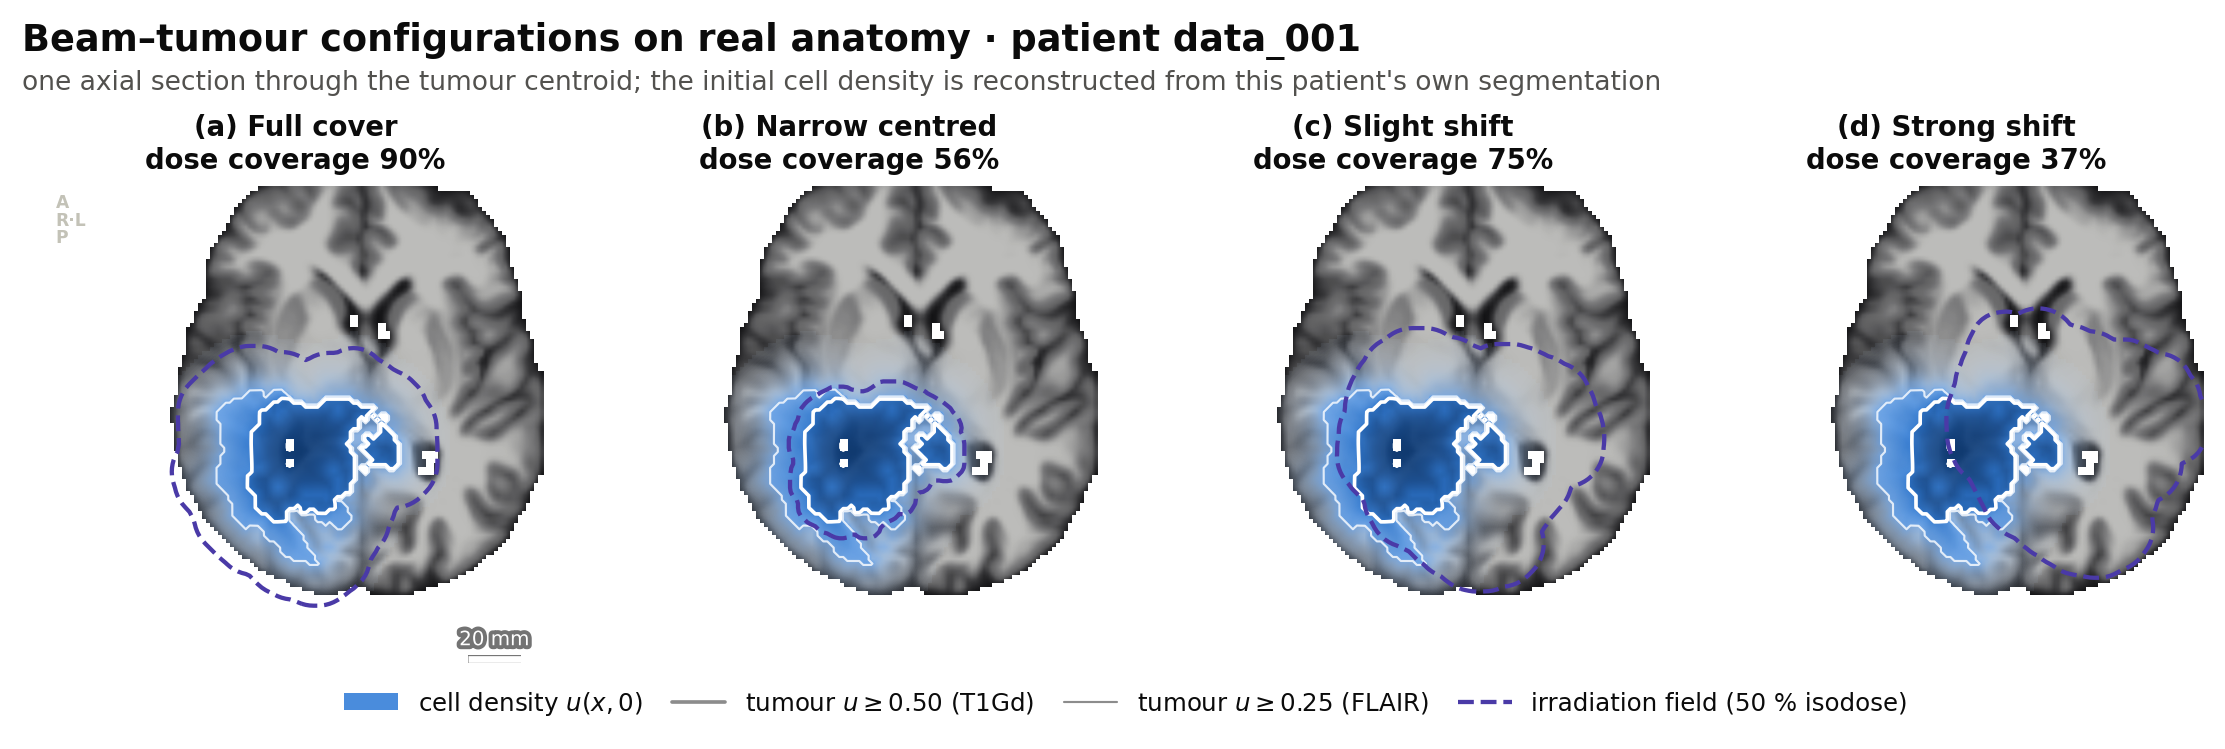
\includegraphics[width=1.0\textwidth]{figures/f3_beam_configs.png}
\caption{The four beam--tumour configurations on one patient's real anatomy.
White contours are the reconstructed tumour iso-surfaces at $u=0.50$ (T1Gd) and
$u=0.25$ (FLAIR); the dashed contour is the 50\,\% isodose. Coverage is the
mass-weighted fraction of tumour inside the field.}
\label{fig:beam_configs}\end{figure}

\begin{figure}[t]\centering
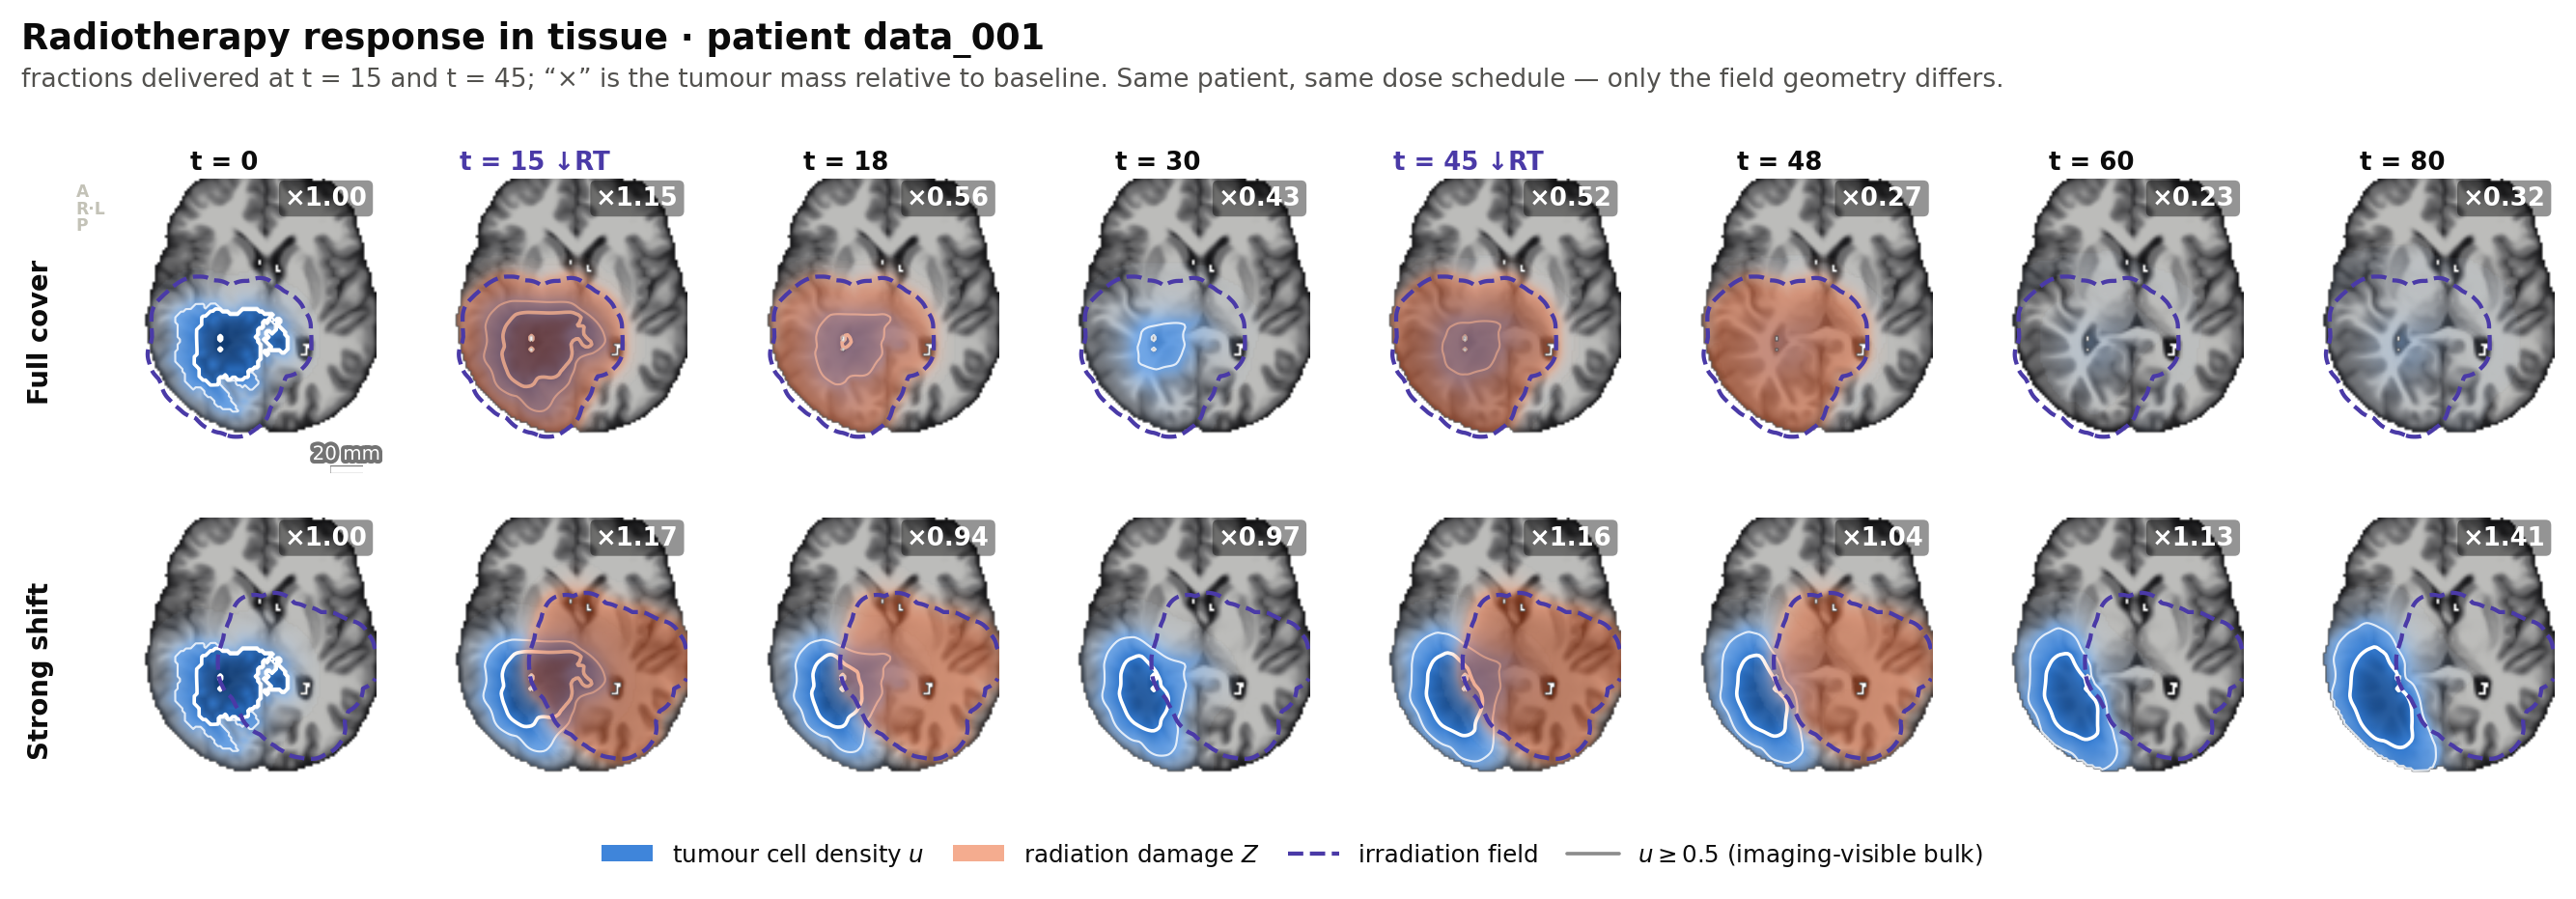
\includegraphics[width=1.0\textwidth]{figures/f4_time_evolution.png}
\caption{Spatial radiotherapy response for one patient: the same dose schedule
under two field geometries. Blue is tumour cell density, orange the
radiation-damage field $Z$, and the annotation is tumour mass relative to
baseline. Under full cover the tumour is driven to a fraction of its initial
mass; under the displaced field the untreated shoulder survives and regrows.}
\label{fig:time_evolution}\end{figure}

\begin{figure}[t]\centering
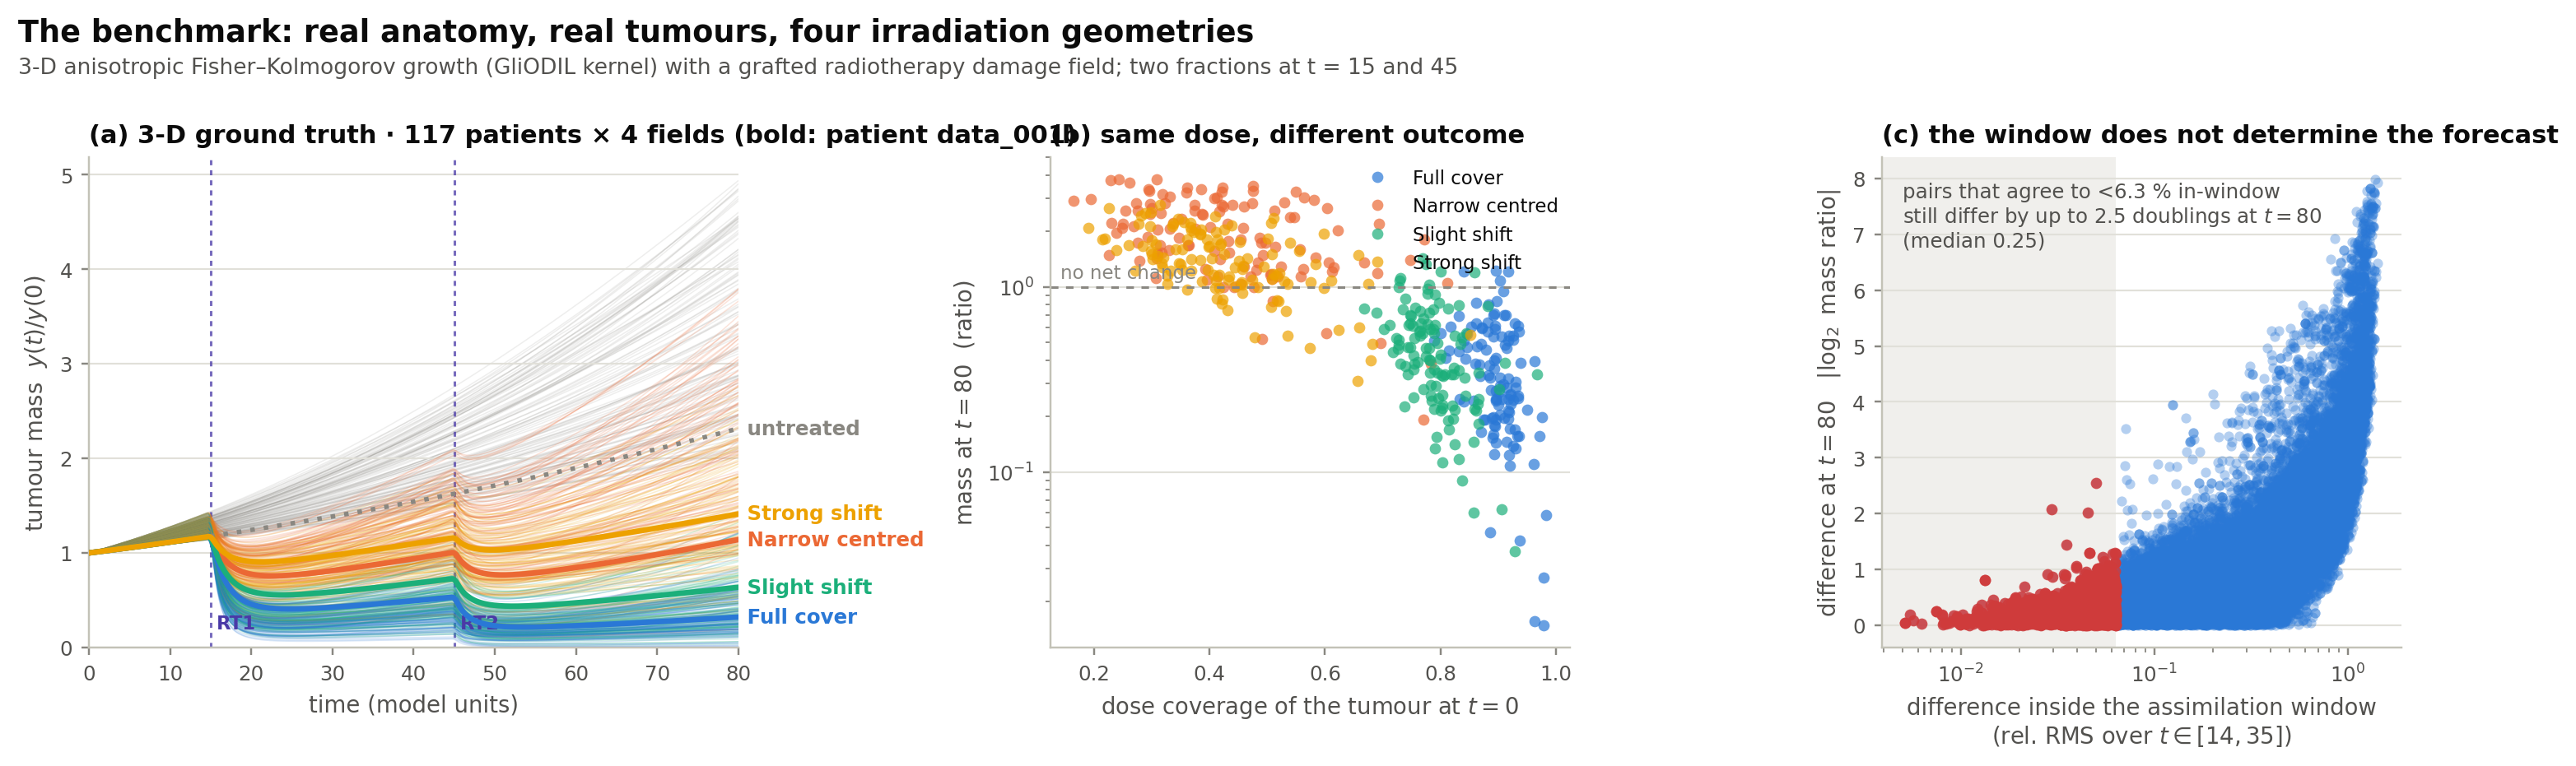
\includegraphics[width=1.0\textwidth]{figures/f1_ground_truth.png}
\caption{(a) Reference mass trajectories for all 117 patients and four
geometries. (b) Delivered dose against outcome. (c) The premise of the study,
quantified: pairs of trajectories that agree closely inside the assimilation
window still diverge by up to several doublings at $t=80$, so the window alone
does not determine the forecast.}
\label{fig:ground_truth}\end{figure}

\subsection{Assimilation Protocol}

For every (patient, configuration) pair we draw $N_{\mathrm{fit}}=20$ evenly
spaced observations on $[14,35]$ --- one time unit earlier than
Table~\ref{tab:assimilation} so that the window brackets the whole first
fraction rather than beginning on it --- perturb them with
$\mathcal{N}\bigl(0,(0.02\,y_i)^2\bigr)$ noise in 20 independent realisations,
and forecast $(35,80]$, which contains the second, unseen irradiation event.
This gives $468$ patient--configuration columns and
$20468$ independently fitted models per method.

All surrogates share one fitting procedure: the same batched fourth-order
Runge--Kutta integrator on a fixed refined grid (decoupled from the observation
times, so a fitted parameter cannot depend on how densely the tumour happened to
be measured), the same optimiser and budget, and the same number of random
restarts. Differences in accuracy are therefore differences between models, not
between fitting procedures.

\paragraph{Compute.}
The unrolled Runge--Kutta loop over a two-state system is kernel-launch bound
rather than compute bound, so batch width is almost free: widening the batch
$22\times$ costs $1.4\times$ the wall-clock. Every method is therefore fitted for
the entire cohort in one tensor whose batch axis carries
(patient $\times$ configuration $\times$ noise realisation $\times$ restart) ---
of order $10^{4}$ independent reduced models trained simultaneously per method.
The reported experiments were run on eight NVIDIA RTX 6000 Ada GPUs, two worker
processes per device.

\subsection{The Growth Law Implied by the Reference Dynamics}

Before comparing surrogates it is worth checking which reduced growth law the
three-dimensional reference actually follows, since this is a property of the
data and not of any surrogate. On the untreated trajectories, $y^{1/3}$ is
linear in $t$ with median $R^{2}=0.9995$, against $0.9864$ for the mass
itself, and the effective exponent recovered from
$\mathrm{d}\log\dot y/\mathrm{d}\log y$ has median $0.81$
($0.65$--$0.90$ over the cohort). This confirms
Eq.~\eqref{eq:volumetric_rate} empirically and locates the truth between the
surface-growth exponent $2/3$ and the logistic exponent $1$, distinctly away
from the latter (Fig.~\ref{fig:growth_law}).

\begin{figure}[t]\centering
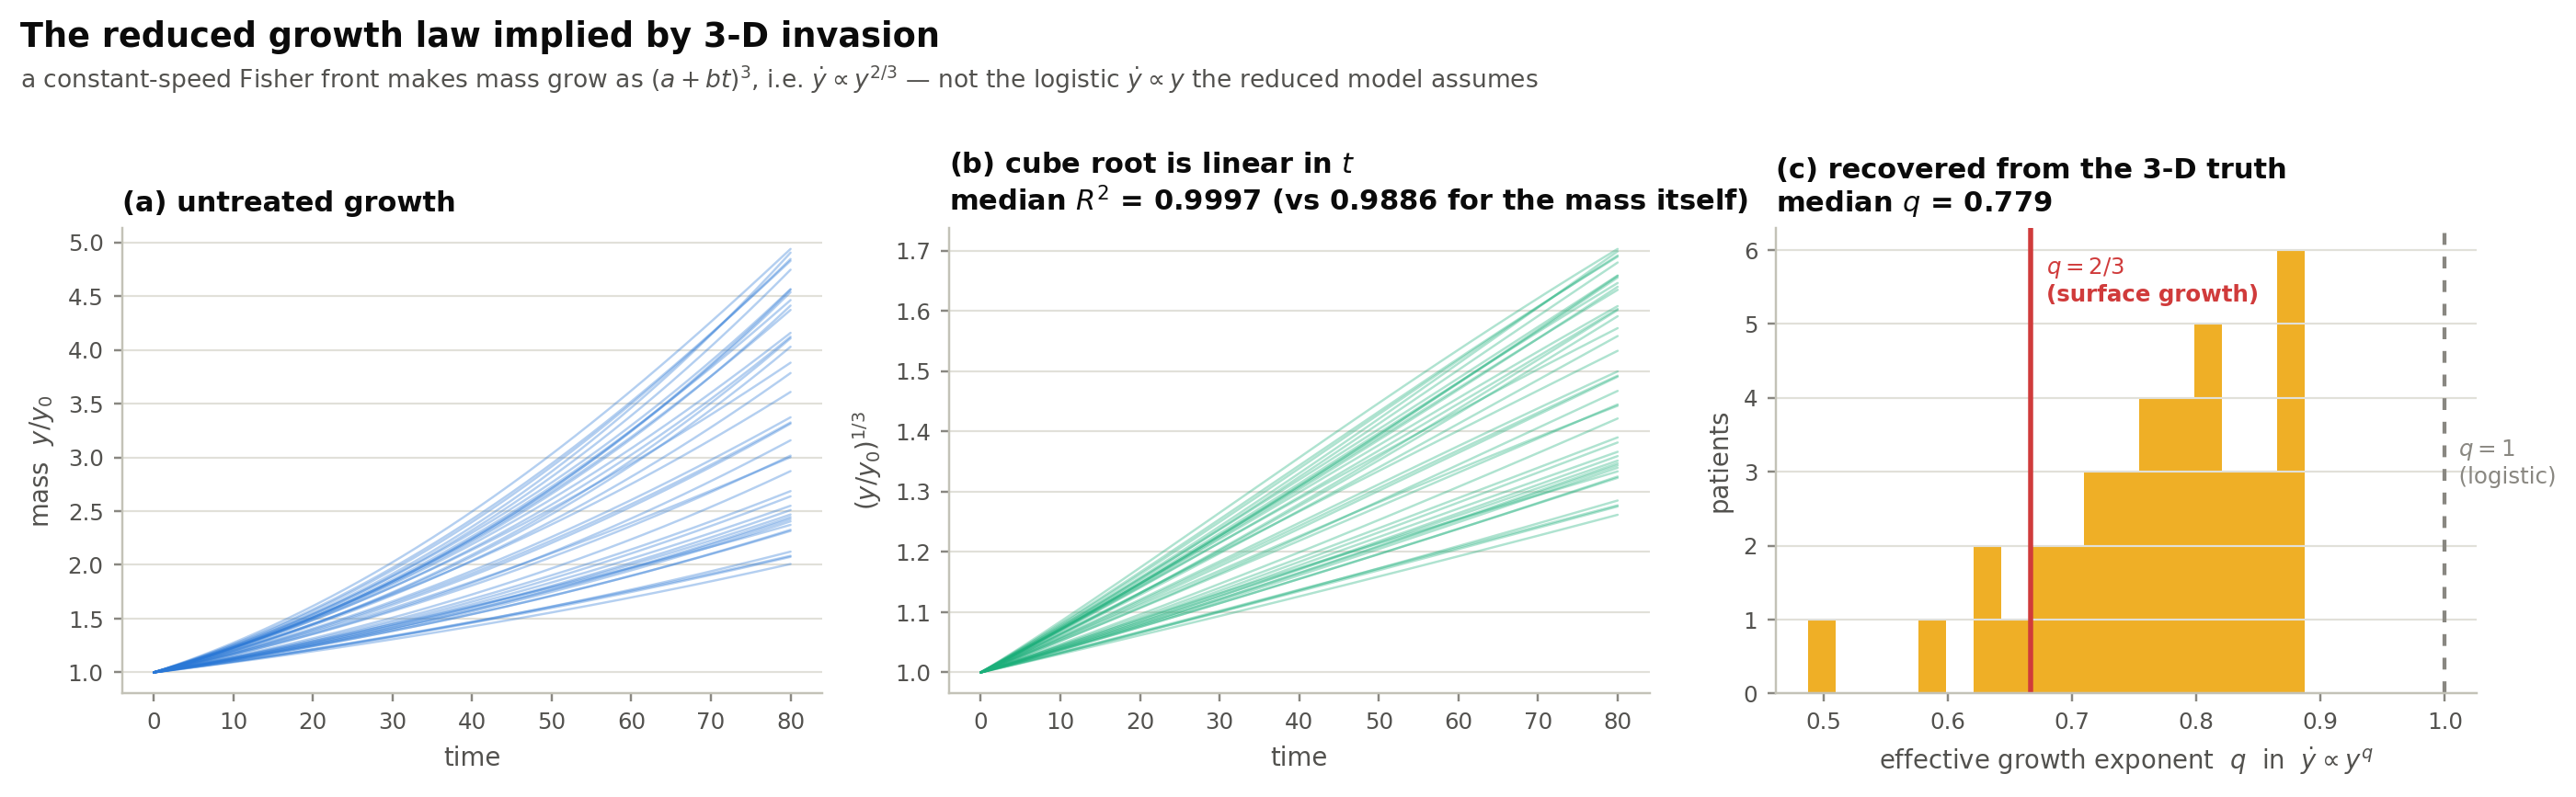
\includegraphics[width=1.0\textwidth]{figures/f2_growth_law.png}
\caption{The reduced growth law implied by three-dimensional invasion.
(a) Untreated reference trajectories. (b) Their cube roots, which are linear in
time. (c) The effective growth exponent $q$ recovered per patient, against the
surface-growth value $2/3$ and the logistic value $1$.}
\label{fig:growth_law}\end{figure}

\subsection{How Much of the Gap Is Structural?}

A forecast error mixes two things: what the reduced model \emph{cannot
represent}, and what it \emph{cannot infer} from twenty noisy samples. We
separate them by fitting each backbone a second time to the entire noise-free
trajectory over $[14,80]$ --- an oracle with no estimation error at all. The
residual of that fit is the irreducible closure gap, and it is exactly the
quantity a learned closure exists to absorb.
